%	PACKAGES AND OTHER DOCUMENT CONFIGURATIONS

\documentclass[11pt, a4paper]{article} % 10pt font size (11 and 12 also possible), A4 paper (letterpaper for US letter) and two column layout (remove for one column) Use additional titlepage argument to generate this
%\documentclass[12pt, a4paper,twocolumn,titlepage]{article}

%%%%%%%%%%%%%%%%%%%%%%%%%%%%%%%%%%%%%%%%%
% Wenneker Article
% Structure Specification File
% Version 1.0 (28/2/17)
%
% This file originates from:
% http://www.LaTeXTemplates.com
%
% Authors:
% Frits Wenneker
% Vel (vel@LaTeXTemplates.com)
%
% License:
% CC BY-NC-SA 3.0 (http://creativecommons.org/licenses/by-nc-sa/3.0/)
%
%%%%%%%%%%%%%%%%%%%%%%%%%%%%%%%%%%%%%%%%%

%----------------------------------------------------------------------------------------
%	PACKAGES AND OTHER DOCUMENT CONFIGURATIONS
%----------------------------------------------------------------------------------------

\usepackage[english]{babel} % English language hyphenation

\usepackage{microtype} % Better typography

\usepackage{verbatim} % Allows mulitline commenting

\usepackage{amsmath,amsfonts,amsthm} % Math packages for equations

\usepackage[svgnames]{xcolor} % Enabling colors by their 'svgnames'

\usepackage[hang, small, labelfont=bf, up, textfont=it]{caption} % Custom captions under/above tables and figures

\usepackage{subcaption}

\usepackage{booktabs} % Horizontal rules in tables

\usepackage{lastpage} % Used to determine the number of pages in the document (for "Page X of Total")

\usepackage{graphicx} % Required for adding images

\usepackage{enumitem} % Required for customising lists
\setlist{noitemsep} % Remove spacing between bullet/numbered list elements

\usepackage{sectsty} % Enables custom section titles
\allsectionsfont{\usefont{OT1}{phv}{b}{n}} % Change the font of all section commands (Helvetica)

\usepackage{siunitx}

%----------------------------------------------------------------------------------------
%	MARGINS AND SPACING
%----------------------------------------------------------------------------------------

\usepackage{geometry} % Required for adjusting page dimensions

\geometry{
	top=1cm, % Top margin
	bottom=1.5cm, % Bottom margin
	left=2cm, % Left margin
	right=2cm, % Right margin
	includehead, % Include space for a header
	includefoot, % Include space for a footer
	%showframe, % Uncomment to show how the type block is set on the page
}

\setlength{\columnsep}{7mm} % Column separation width

%----------------------------------------------------------------------------------------
%	FONTS
%----------------------------------------------------------------------------------------

\usepackage[T1]{fontenc} % Output font encoding for international characters
\usepackage[utf8]{inputenc} % Required for inputting international characters

\usepackage{XCharter} % Use the XCharter font

%----------------------------------------------------------------------------------------
%	HEADERS AND FOOTERS
%----------------------------------------------------------------------------------------

\usepackage{fancyhdr} % Needed to define custom headers/footers
\pagestyle{fancy} % Enables the custom headers/footers

\renewcommand{\headrulewidth}{0.0pt} % No header rule
\renewcommand{\footrulewidth}{0.4pt} % Thin footer rule

\renewcommand{\sectionmark}[1]{\markboth{#1}{}} % Removes the section number from the header when \leftmark is used

%\nouppercase\leftmark % Add this to one of the lines below if you want a section title in the header/footer

% Headers
\lhead{} % Left header
\chead{\textit{\thetitle}} % Center header - currently printing the article title
\rhead{} % Right header

% Footers
\lfoot{} % Left footer
\cfoot{} % Center footer
\rfoot{\footnotesize Page \thepage\ of \pageref{LastPage}} % Right footer, "Page 1 of 2"

\fancypagestyle{firstpage}{ % Page style for the first page with the title
	\fancyhf{}
	\renewcommand{\footrulewidth}{0pt} % Suppress footer rule
}

%----------------------------------------------------------------------------------------
%	TITLE SECTION
%----------------------------------------------------------------------------------------

\newcommand{\authorstyle}[1]{{\large\usefont{OT1}{phv}{b}{n}\color{NavyBlue}#1}} % Authors style (Helvetica)

\newcommand{\institution}[1]{{\footnotesize\usefont{OT1}{phv}{m}{sl}\color{Black}#1}} % Institutions style (Helvetica)

\usepackage{titling} % Allows custom title configuration

\newcommand{\HorRule}{\color{SteelBlue}\rule{\linewidth}{1pt}} % Defines the gold horizontal rule around the title

\pretitle{
	\vspace{-30pt} % Move the entire title section up
	\HorRule\vspace{10pt} % Horizontal rule before the title
	\fontsize{32}{36}\usefont{OT1}{phv}{b}{n}\selectfont % Helvetica
	\color{Navy} % Text colour for the title and author(s)
}

\posttitle{\par\vskip 15pt} % Whitespace under the title

\preauthor{} % Anything that will appear before \author is printed

\postauthor{ % Anything that will appear after \author is printed
	\vspace{10pt} % Space before the rule
	\par\HorRule % Horizontal rule after the title
	\vspace{20pt} % Space after the title section
}

%----------------------------------------------------------------------------------------
%	ABSTRACT
%----------------------------------------------------------------------------------------

\usepackage{lettrine} % Package to accentuate the first letter of the text (lettrine)
\usepackage{fix-cm}	% Fixes the height of the lettrine

\newcommand{\initial}[1]{ % Defines the command and style for the lettrine
	\lettrine[lines=3,findent=4pt,nindent=0pt]{% Lettrine takes up 3 lines, the text to the right of it is indented 4pt and further indenting of lines 2+ is stopped
		\color{NavyBlue}% Lettrine colour gold DarkGoldenRod
		{#1}% The letter
	}{}%
}

\usepackage{xstring} % Required for string manipulation

\newcommand{\lettrineabstract}[1]{
	\StrLeft{#1}{1}[\firstletter] % Capture the first letter of the abstract for the lettrine
	\initial{\firstletter}\textbf{\StrGobbleLeft{#1}{1}} % Print the abstract with the first letter as a lettrine and the rest in bold
}

%	BIBLIOGRAPHY

\usepackage[backend=biber,style=phys,natbib=true,doi=false]{biblatex} 
%Can equally use numeric citation style without extra phys packaging (but doesn't change capitalisation), or authoryear for alphabetical listing without the codes (resembles APA)

%\addbibresource{references.bib} % The filename of the bibliography

\usepackage[autostyle=true]{csquotes} % Required to generate language-dependent quotes in the bibliography

%    APPENDICES

\usepackage[title]{appendix} %in appendix


 % Specifies the document structure and loads requires packages
\usepackage{graphicx}
\graphicspath{{../Figures/}}
\newcommand*{\subscript}[1]{\ensuremath{_\textrm{{\scriptsize #1}}}}

%	ARTICLE INFORMATION

\title{Simulating Liquid Crystals}

%\author{
	%\authorstyle{Christopher Gallagher}}
\author{\authorstyle{Kit Gallagher} 
	%\institution{University of Cambridge \\
	\institution{Supervisors: Prof Erika Eiser, Mr Jiaming Yu}}
% Example of a one line author/institution relationship
%\author{\newauthor{John Marston} \newinstitution{Universidad Nacional Autónoma de México, Mexico City, Mexico}}

\date{\today} % Add a date here if you would like one to appear underneath the title block, use \today for the current date, leave empty for no date
\usepackage[english]{babel}
\usepackage{tabularx}
%\renewcommand{\thefootnote}{\roman{footnote}}  %use roman lettering for footnotes instead
\usepackage[backend=biber,doi=false]{biblatex}
\addbibresource{reportreferences.bib}
%\AtBeginBibliography{\small}
%----------------------------------------------------------------------------------------
\begin{document}

\maketitle % Print the title

\thispagestyle{firstpage} % Apply the page style for the first page (no headers and footers)

%	ABSTRACT

\lettrineabstract{This document is simply to give an overview of methods used and data obtained in the project. It is likely that many of the methods and results detailed here will be used in the final report, but this is not intended to be a full report; rather a collection of ideas that can be used in the writing of this final report.} 




%	ARTICLE CONTENTS
\section{Methods}
\subsection{Order Parameter} \label{Order_param_theory}
\textit{"The description of liquid crystals involves an analysis of order. A second rank symmetric traceless tensor order parameter is used to describe the orientational order of a nematic liquid crystal, although a scalar order parameter is usually sufficient to describe uniaxial nematic liquid crystals. To make this quantitative, an orientational order parameter is usually defined based on the average of the second Legendre polynomial:}

\begin{equation}
 S=\langle P_{2}(\cos \theta )\rangle =\left\langle {\frac {3\cos ^{2}(\theta )-1}{2}}\right\rangle
\end{equation}
\textit{where $\theta$ is the angle between the liquid-crystal molecular axis and the local director (which is the 'preferred direction' in a volume element of a liquid crystal sample, also representing its local optical axis)."} - Copied from wiki

However, in our case the local director is not known, and so I have approximated it as the mean director averaged across all particles. Eppenga et al. \cite{Eppenga1984} suggest an alternative method, for when this local director is not known.

\section{Results}
\subsection{Square Simulation Region}
This section details the results from my first long simulation to achieve nematic phase formation. This simulation took three hours to run, and consisted of 6 shrinking stages (each of 50,000 steps), with 1,000,000 simulation steps between each one. It had 1000 particles inside a cubic box, of initial side length 10 times greater than the length of one nanoparticle. The final side length of the box was 2.5 times greater than the length of one nanoparticle, with a final volume fraction within the box of X\%.%haven't decided how to quantify this

After the penultimate shrinking step, a phase transition was observed from the disordered isotropic phase to an ordered nematic phase, as depicted in Figure \ref{fig:cubic_particles}. This is characterised by orientational order (ie particles tend to have similar orientations), while having no long range positional order (ie the centres of mass of each particle are randomly distributed through space). This can be observed easily in Figure \ref{fig:cubic_nematic}, where particle ordering can be easily observed on the top and right hand faces. Note that each molecule is artificially given a different colour to aid recognition of them; this does not have any physical relevance.

\begin{figure}[ht]
	\begin{subfigure}{.45\textwidth}
		\centering
		% include first image
		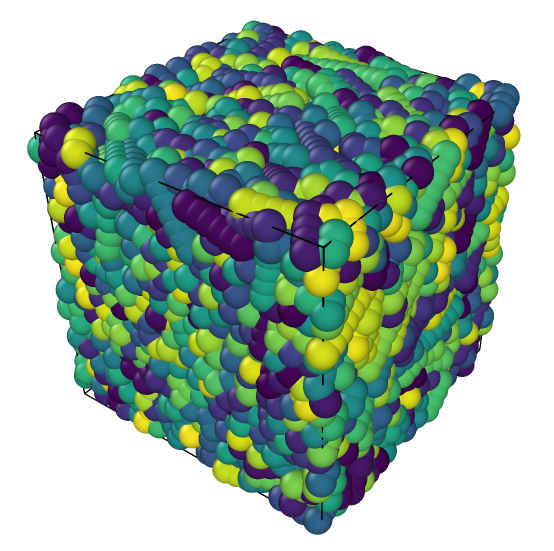
\includegraphics[width=\linewidth]{Figures/longrun_phasetrans2}  
		\caption{Liquid State}
		\label{fig:cubic_liquid}
	\end{subfigure}
	\hfill %% useful if width of each figure is less the .5\textwidth
	\begin{subfigure}{.42\textwidth} %lower so both figs are same size
		\centering
		% include second image
		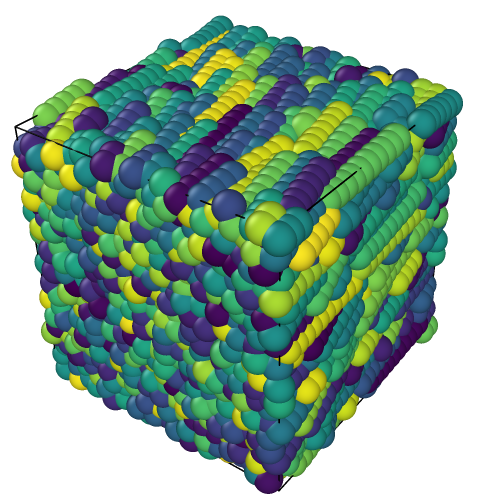
\includegraphics[width=\linewidth]{Figures/longrun_phasetrans3}  
		\caption{Nematic State}
		\label{fig:cubic_nematic}
	\end{subfigure}
	\caption{Comparison between phase appearance, before an after the nematic phase transition. Note the common alignment in the nematic phase, without positional order.}
	\label{fig:cubic_particles}
\end{figure}

This phase transition is most easily observed through a jump in the pressure of the system. The equilibrium pressure at various volume fractions is plotted in Figure \ref{fig:cubic_pressure_phase}, displaying a steep change around the critical volume fraction. It is predicted that this curve would flatten out when extended over sufficiently long regions, however in this system the phase transition occurs too close to the maximal volume fraction for this to be observed. 

%This is the story that jiaming has told me. However I am not sure if it is true; we would expect the pressure to increase (as a 1/V relation for an ideal gas) as the system is compressed and so this is observed. The formation of a new phase actually corresponds to a decrease in pressure, and so is not responsible for this sharp increase. Furthermore, Jiaming expects this curve to flatten out, but I am not sure this is even possible.

The evolution of pressure is displayed as the system equilibrates after each shrinking stage in Figure \ref{fig:cubic_pressure_evo}. It is particularly notable here that pressure is expected to be constant under the nve ensemble (given the additional presence of a temperature thermostat), and this is indeed observed at low volume fractions (corresponding to smaller values of 'mix\_steps' - the shrinking time). However, there is a clear phase transition occurring during the fourth shrinking section, with a decrease in the pressure of the red curve. The phase transition may not be complete after this step, hence the smaller pressure change in the next equilibration stage (following further shrinking), given in the purple line. 

\begin{figure}[ht]
	\centering
	\begin{minipage}[b]{0.45\textwidth}
		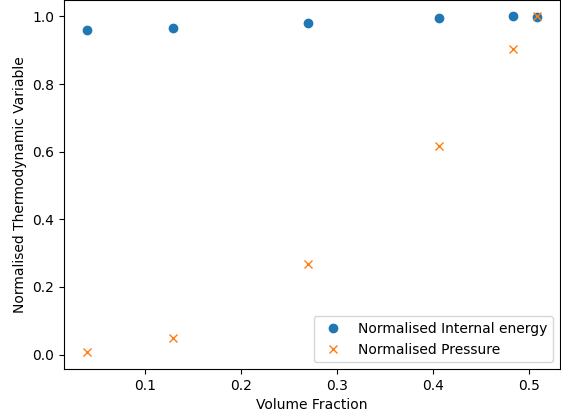
\includegraphics[width=\linewidth]{Figures/phaseplot_frac_cubic}  
		\caption{Evolution of thermodynamic variables over time; change in pressure corresponds to phase transition.}
		\label{fig:cubic_pressure_phase}
	\end{minipage}
	\hfill
	\begin{minipage}[b]{0.45\textwidth}
		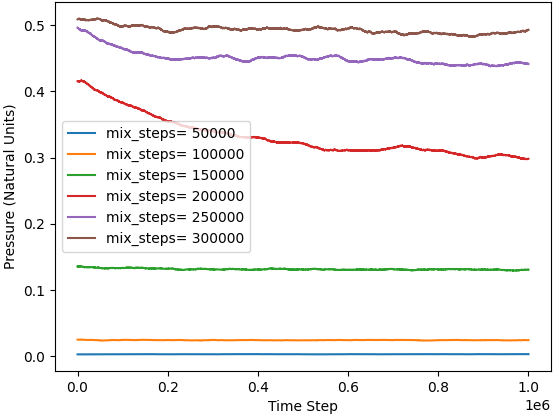
\includegraphics[width=\linewidth]{Figures/pressureplot_frac_cubic}  
		\caption{Pressure evolution when system is equilibrating; the change in the red curve denotes a phase transition over this run.}
		\label{fig:cubic_pressure_evo}
	\end{minipage}
\end{figure}

It is a time average of these curves that gives the pressures used in Figure \ref{fig:cubic_pressure_phase}, although only the last 10\% of the curve is used, where the system is assumed to have finished equilibrating, to give an accurate measurement of temperature. It should be noted however that the pressure is hard to define in molecular level systems like this, and is subject to significant fluctuations due to its low magnitude. This meant that the curves in \ref{fig:cubic_pressure_evo} have been smoothed significantly, and are subject to variations much greater than their net change, on the order of $\pm 0.1$ natural units.

It is for this reason that an alternative method to quantify the phase change here is sought. Traditionally the order parameter is used for the nematic phase change, detailed in Section \ref{Order_param_theory}. This was calculated (approximating the local director as the mean molecular axis) and plotted against volume fraction in Figure \ref{fig:cubic_order}. It should be noted that the absolute value of the order parameter is plotted here, as negative values were observed.

\begin{figure}
	\centering
	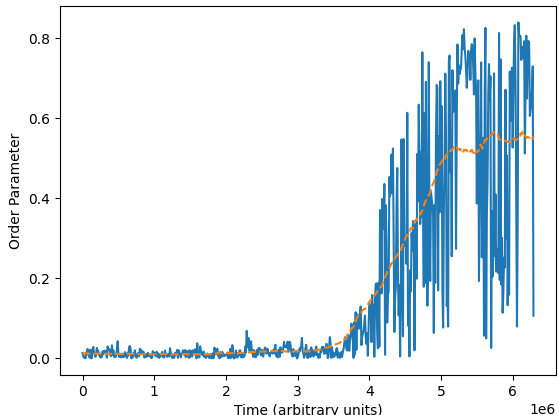
\includegraphics[width=0.7\linewidth]{Figures/director_evo_cubic}
	\caption{The evolution of the order parameter over time for the rigid rod system depicted in blue. A rolling average (calculated over a uniform window of 500 steps) is superimposed in red here to display the overall increase in this value, and the distinct change around 4.5 million steps}
	\label{fig:cubic_order}
\end{figure}

Further work here will extend this to an oblong simulation region, to aid the formation of ordered phases.

\subsection{Oblong Simulation Region}
Typically, the formation of ordered phase structures such as nematic or smectic phases is impeded by the edge effects of the box; the periodic boundary conditions here can destabilise the formation of ordered phases if the simulation dimensions are not an integer multiple of the molecule dimensions. (For example, when forming a smectic phase the molecules cannot line up fully in columns and must overlap at the edges of the box.)

This effect is mitigated by increasing the volume of the simulation box, as the overlapping regions form a smaller proportion of the overall structure (and this overlap may be distributed further to reduce the energy cost). We typically aim for a simulation region 5/6 larger than the molecular dimension. However, a larger simulation regions comes with associated computational costs, as a greater number of molecules are required to achieve the same volume fraction.

These costs can be reduced by breaking the symmetry of the system; we may be introduce a long axis in our simulation region to generate an oblong box. Ordered phases will preferentially form along this long axis, as the energy costs associated with the boundaries are reduced. In this way the number of particles required to 'fill' the box (i.e. achieve the desired volume fraction) is minimised, while retaining the longer simulation axis for ordered phase formation.

The simulation region is therefore adjusted to have a 3:1:1 aspect ratio, with the same time steps as used previously.The final phase structure formed depicted in Figure \ref{fig:oblong_structure}, and displays multiple regions of nematic phase with differing directors. The origin for this phase structure is unknown, but introduces complexity when identifying the critical volume fraction of the phase transition.

\begin{figure}
	\centering
	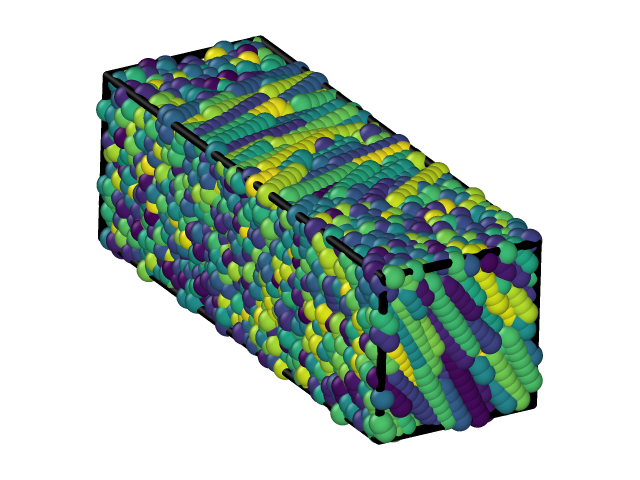
\includegraphics[width=0.7\linewidth]{Figures/longrun2_oblong}
	\caption{The ordered phase formed in the oblong simulation region; note the two different sections of nematic phase in the foreground and background of the image, with varying local director orientations.}
	\label{fig:oblong_structure}
\end{figure}

Further long-time simulations, with 18 shrinking sections of 25000 steps and 500,000 equilibration steps between each one, were conducted to identify the phase transition more accurately. 

\begin{figure}[ht]
	\centering
	\begin{minipage}[b]{0.45\textwidth}
		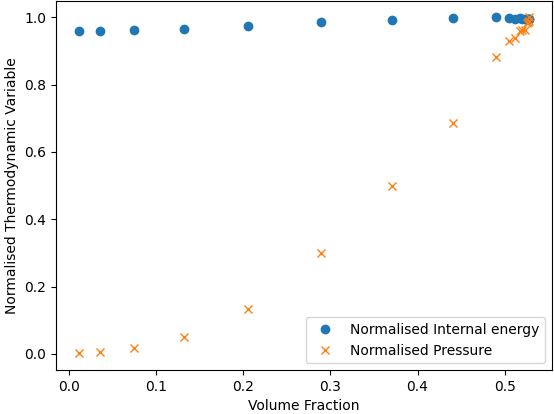
\includegraphics[width=\linewidth]{Figures/phaseplot_frac_oblong}  
		\caption{Evolution of thermodynamic variables over time; change in pressure corresponds to phase transition. Note the cluster of points at high pressures corresponding to the limit of maximal volume fraction.}
		\label{fig:oblong_pressure_phase}
	\end{minipage}
	\hfill
	\begin{minipage}[b]{0.45\textwidth}
		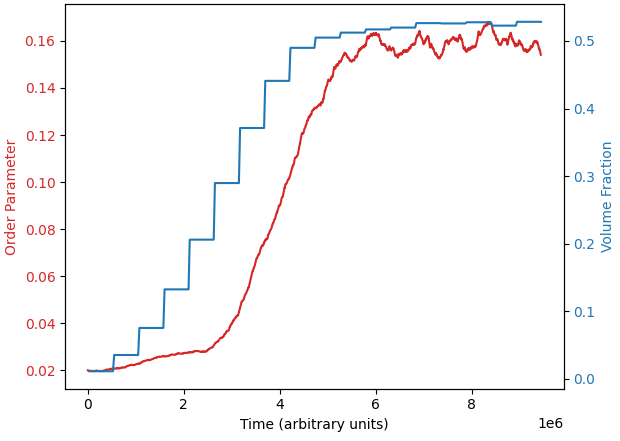
\includegraphics[width=\linewidth]{Figures/order_and_volfrac_oblong}  
		\caption{Evolution of the order parameter and volume fraction over time; note the steep change in order parameter at median times, and the subsequent levelling off suggesting  a new phase has been reached.}
		\label{fig:oblong_order_evo}
	\end{minipage}
\end{figure}

Again thermodynamic variables have been recorded over time here. It is particularly telling that the points cluster at high pressures in Figure \ref{fig:oblong_pressure_phase}; this indicates that we are approaching the maximal volume fraction and further compression is not possible here, hence it is unlikely we will observe this section of the graph levelling off.

A quasi-discrete change in order parameter is observed clearly in this system as the volume fraction increases, depicted in Figure \ref{fig:oblong_order_evo}. Again smoothing is required to obtain this order parameter, and the absolute value must be taken to avoid negative values. These suggest that mean value approach to calculate the local director may not be valid, and a more advanced method will be implemented for future simulations.

%\clearpage
\printbibliography

\end{document}


%%%%%%%%%%%%%%%%%%%%%%%%%%%%%%%%%%%%%%%%%
% Wenneker Article
% LaTeX Template
% Version 2.0 (28/2/17)
%
% This template was downloaded from:
% http://www.LaTeXTemplates.com
%
% Authors:
% Vel (vel@LaTeXTemplates.com)
% Frits Wenneker
%
% License:
% CC BY-NC-SA 3.0 (http://creativecommons.org/licenses/by-nc-sa/3.0/)
%
%%%%%%%%%%%%%%%%%%%%%%%%%%%%%%%%%%%%%%%%%
